\chapter{I Asked Californian Millionaires How Much Money They Lost}

We begin in the street, not at a blackboard. Luxury cars, quick questions, and abrupt numbers create the first impression, but the real object of the lecture is sharper: how gains are made, why gains reverse, what kind of mechanism sits behind the reversal, and what habits survive the reversal. These notes keep the interview order intact and extract the small but real mathematical spine of the episode: performance pay, repeated asset accumulation, delegation as a scaling condition, liquidity mismatch, and the contrast between additive effort and compounding effort.

\section{Opening Premise: Wealth and Fragility}

The transcript opens with a teaser-like glimpse of the final boom-and-bust story and then restarts in Beverly Hills. It is useful to treat that opening as an overture. The governing question is already on the table: not merely who made a great deal of money, but what happened to that money when conditions changed.

The lecture's first quantitative bank is small and concrete:
\begin{equation}
Y_{\mathrm{AI}}=\$40\,\mathrm{M},\qquad
Y_{\mathrm{broker}}\approx \$8\,\mathrm{M},\qquad
Y_{\mathrm{Meltzer}}=\$34\,\mathrm{M},\qquad
L_{\mathrm{Meltzer}}>\$100\,\mathrm{M}.
\end{equation}
These are not yet a theory. They are the lecture's raw observables.

\begin{table}[h]
\centering
\begin{tabular}{lll}
\hline
Case & Peak annual figure & Stress signal or lesson \\
\hline
AI entrepreneur & \(\$40\,\mathrm{M}\) & later loss of \(95\%\) of skincare proceeds \\
Moderate real-estate operator & seven figures & doubles and singles, not only home runs \\
G-Wagon real-estate broker & \(\approx \$8\,\mathrm{M}\) & buy, rent, repeat; delegate to scale \\
David Meltzer & \(\$34\,\mathrm{M}\) & loss \(>\$100\,\mathrm{M}\); stay in business \\
\hline
\end{tabular}
\caption{Transcript-backed gain, loss, and operating signals.}
\end{table}

What matters for the chapter is the rhythm in which these figures are introduced. The host repeatedly asks: what did you make, what happened that year, what did you lose, what would you tell someone starting from nothing? The lecture is therefore structured not as a continuous doctrine, but as a sequence of local models under stress.

\section{The Lamborghini Case: Incentives and Exposure}

The first full case is deliberately extreme. An entrepreneur says he has been in business for eleven years and reports a \(\$40\,\mathrm{M}\) year. The host immediately asks for advice, and the answer is not gradualist. It is a performance-pay doctrine.

In a cleaned-up notation, the example offered in the interview is
\begin{equation}
C=\alpha R,\qquad \alpha \approx \frac12,
\end{equation}
where \(R\) is the revenue one produces for the firm and \(C\) is the commission paid back to the producer. The speaker's rhetoric is strong, but the formal point is clear: the fixed component is suppressed, the variable component is made dominant, and risk is pushed back onto the individual.

A minimal consequence of this model is
\begin{equation}
R=0 \Longrightarrow C=0,
\qquad
R\ \text{large} \Longrightarrow C\propto R.
\end{equation}
The lecture does not present this as a theorem, and we should not rewrite it as one. But it is the operating equation implicitly being defended.

The next move is crucial. The lecture refuses to leave this at the level of heroic earnings. The same interview turns toward scarcity, eviction, a repossessed car, negative bank balance, and the collapse of earlier businesses. The episode insists that upside and exposure belong to the same picture. Later in the same case the speaker reports that he lost \(95\%\) of the money from a skincare sale, which we may record as
\begin{equation}
L_{\mathrm{skin}}=0.95\,Y_{\mathrm{skin}}.
\end{equation}
Again, this is not an abstract formula from finance; it is the transcript's way of forcing us to look at drawdown rather than revenue alone.

\subsection{Question \& Answer}

The lecture now raises its first real obstacle: what can someone at rock bottom actually do? The answer is not a balance-sheet identity. It is a sequence.

\begin{enumerate}
\item Read aggressively in sales, business, and self-reconstruction.
\item Recover a sense of agency; the speaker uses the language of controlling one's reality more than one thinks.
\item Find mentors.
\item Replace a stagnant peer environment with a deliberately chosen one.
\end{enumerate}

The mathematical content here is slight but the sequencing matters. The lecture moves from inner state to social structure. It does not say merely ``work harder.'' It says that the environment in which one learns and the people from whom one learns can change the trajectory of future cash flow and future judgment.

\section{Moderate Real Estate: Risks, Singles, and Beginner Advice}

The next case lowers the temperature. A real-estate operator with decades in business gives advice that is almost opposite in tone to the prior commission-only absolutism. We hear: take risks, yes, but do not insist on the home run every time.

The phrase ``doubles and singles only'' matters because it introduces a different optimization principle. We are no longer maximizing drama. We are maximizing repeatability. The lecture does not give a formal expected-value calculation, but the intended contrast is plain: frequent, survivable gains dominate fantasies of rare, spectacular hits if the cost of a miss is existential.

This is also where the lecture becomes educational in a quieter way. The same operator says that every person one does business with can teach something. That is less a formula than a discipline of accumulation. It fits the lecture's general movement from headline wealth to repeatable practice.

\subsection{Question \& Answer}

The host now asks the beginner's question again, but in a different register: what can someone do coming out of school, broke, and trying to become financially free?

The answer is austere:
\begin{itemize}
\item work hard and do well in school,
\item treat any job as a real job,
\item learn something from everybody with whom you do business.
\end{itemize}

The lecture deliberately resists glamour at this point. After spectacular cars and eight-figure claims, it inserts a plain rule: learning is not postponed until the ideal role arrives. The spoken rhythm is important here. The lecture cools itself on purpose before it escalates again.

\section{The Asset Flywheel and the Limits of Solo Work}

With the G-Wagon case the lecture finally gives us something close to an algorithm. The advice is explicit: buy a property, rent it out, buy another, repeat, and let the income stream rather than the wage stream carry the vehicle payment.

\begin{definition}
We shall call this transcript-derived mechanism the asset flywheel: acquired assets generate cash flow, cash flow supports further acquisition, and only after repetition does consumption become defensible.
\end{definition}

A cautious standard reconstruction is
\begin{align}
P_{n+1} &= P_n + 1,\\
F_{n+1} &= F_n + r_{n+1},
\end{align}
where \(P_n\) is the number of properties after year \(n\), \(F_n\) is accumulated passive cash flow, and \(r_{n+1}\) is the cash flow generated by the newly added property.

Let us work this through in the exact spirit of the interview. Start at
\[
P_0=0,\qquad F_0=0.
\]
If one buys one house each year for four years, then
\begin{align}
P_1&=1, & F_1&=r_1,\\
P_2&=2, & F_2&=r_1+r_2,\\
P_3&=3, & F_3&=r_1+r_2+r_3,\\
P_4&=4, & F_4&=r_1+r_2+r_3+r_4.
\end{align}
By the fifth year, the lecture's claim is that this accumulated passive income can be directed toward the vehicle, so the spoken condition becomes
\begin{equation}
F_4 \gtrsim M_{\mathrm{GW}},
\end{equation}
where \(M_{\mathrm{GW}}\) denotes the monthly G-Wagon payment. No rent schedule, mortgage schedule, or vacancy rate is given in the lecture, so we keep the model schematic.

\begin{figure}[h]
\centering
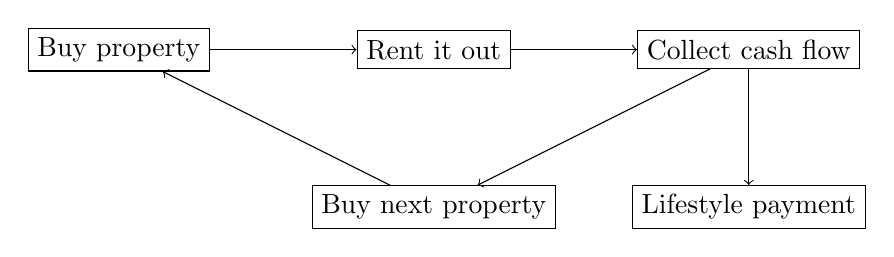
\begin{tikzpicture}[scale=1]
\node[draw, rectangle] (buy) at (0,0) {Buy property};
\node[draw, rectangle] (rent) at (4,0) {Rent it out};
\node[draw, rectangle] (flow) at (8,0) {Collect cash flow};
\node[draw, rectangle] (next) at (4,-2) {Buy next property};
\node[draw, rectangle] (pay) at (8,-2) {Lifestyle payment};

\draw[->] (buy) -- (rent);
\draw[->] (rent) -- (flow);
\draw[->] (flow) -- (next);
\draw[->] (flow) -- (pay);
\draw[->] (next) -- (buy);
\end{tikzpicture}
\caption{Transcript-derived asset flywheel: acquire, rent, accumulate, repeat, and only then consume.}
\end{figure}

The lecture does not stop at the flywheel. It asks the scaling question immediately afterward: if this grows into a large business, how important is delegation?

\subsection{Question \& Answer}

The answer is that scale begins exactly where personal centrality ends. The speaker recalls an entrepreneur who effectively managed by conversation while every other function was carried by someone else. That is the lecture's cleanest statement of organizational scaling:
\begin{equation}
\text{Scale} \Longrightarrow \text{A-to-Z functions are handled by others, not by one operator.}
\end{equation}

The logical sequence is simple.
\begin{enumerate}
\item If one person performs every function, every function shares the same bottleneck.
\item If each function is reassigned to another competent person, the organization is no longer limited by one daily schedule.
\item The difficult skill is therefore not raw effort alone, but hiring, onboarding, and retaining the right people.
\end{enumerate}

This is one of the lecture's strongest transitions. The problem has moved from ``How do we make money?'' to ``How do we prevent growth from collapsing back into one human being?''

\section{David Meltzer: Boom, Credit, and the Survival Constraint}

The final interview is introduced as a special case, and it justifies that treatment. We are now at SoFi Stadium, and the lecture becomes more analytic. The speaker reports a \(\$34\,\mathrm{M}\) year, attributes it to a real-estate boom, and then says that the real estate he owned doubled in one year. In a deliberately cautious notation we may write
\begin{equation}
V_1 \approx 2V_0,
\end{equation}
where \(V_0\) is the marked value of the real-estate position before the boom and \(V_1\) the marked value after it. This is only the speaker's shorthand, not a fully specified valuation model.

The lecture then pivots sharply to the crash. The central mechanism is not merely falling prices; it is a liquidity mismatch:
\begin{align}
C_{\mathrm{nominal}} &= \$40\,\mathrm{M},\\
C_{\mathrm{usable}} &= \$1\,\mathrm{M},\\
N &\approx \$5\,\mathrm{M},\\
C_{\mathrm{usable}} &< N.
\end{align}
This is the cleanest piece of mathematics in the lecture. One may possess a nominal line of credit and still fail at the precise moment when cash is required. The transcript's lesson is not that credit disappeared abstractly; it is that usable credit was smaller than the financing need when the regime changed.

\begin{definition}
The survival constraint is the rule that one must remain in business tomorrow before optimizing for growth today.
\end{definition}

That is the lecture's ``golden rule of business.'' It sounds informal, but its logic is exact. If continuity fails, every later upside is irrelevant. The order of objectives is therefore
\[
\text{survival} \;\; \text{before} \;\; \text{scale} \;\; \text{before} \;\; \text{luxury}.
\]

The speaker adds a retrospective moral to the credit-line story: he should have asked for help from people who really understood financing and banking. The lecture is careful here. Wealth, in the episode, does not imply mastery of every financial sub-problem.

\subsection{Question \& Answer}

The final conceptual question is the most nearly mathematical one: why does consistency compound?

The lecture first sets up a contrast in spoken arithmetic. In our notation,
\begin{align}
A_n &= \underbrace{1+1+\cdots+1}_{n\text{ terms}} = n,\\
G_n &= 1+2+4+\cdots+2^{n-1}.
\end{align}
The point is not that every effort literally doubles. The point is that repeated, daily, organized action behaves differently from isolated bursts.

If we translate the speaker's geometric sketch into a standard derivation, we get
\begin{align}
2G_n &= 2+4+\cdots+2^n,\\
2G_n-G_n &= (2+4+\cdots+2^n)-(1+2+4+\cdots+2^{n-1}),\\
G_n &= 2^n-1.
\end{align}
So additive effort gives
\[
A_n=n,
\]
while the geometric sketch gives
\[
G_n=2^n-1.
\]
The lecture invokes this contrast to explain why ``two minutes a day'' can outperform a heroic but isolated burst on the weekend. The mathematics here is a standard reconstruction of the interview's intuition, not a claim that business outcomes literally follow a pure geometric law.

\begin{remark}
The references to physics, metaphysics, quantum physics, and the rule of \(72\) should be taken cautiously. The clean mathematical core is simply this: repeated action can create accelerating, aggregating, and compounding effects, whereas irregular action tends to accumulate only linearly.
\end{remark}

\section{Summary}

The lecture begins with public spectacle and ends with operational discipline. Along the way it gives us several distinct mechanisms: performance pay tied directly to output, repeated asset purchase tied to rental cash flow, delegated organization as the precondition of scale, usable liquidity as distinct from nominal wealth, and consistency as the habit that turns accumulation into something like compounding.

What the chapter must preserve is not merely the facts that someone made \(\$40\,\mathrm{M}\), someone made \(\$34\,\mathrm{M}\), or someone lost \(>\$100\,\mathrm{M}\). It must preserve the order in which the lecture teaches us to read those facts. First ask what happened. Then ask what failed. Then ask what survives failure. Only after that do the numbers begin to mean anything.